\chapter{Fit Validation}

Due to the fit's complexity and many adjustable parameters, it is important to verify the fit model and that behaves as intended.

\begin{section}{Signal Injection Study}

Signal injetion studies are a useful way to quantify how well the maximum-likelihood fit can extract a potential signal if it is indeed present.
These studies rely on the use of psuedodata experiments.
A single experiment consists of generating psuedodata by fluctuating bin yields around their pre-fit values according to their statistical and systematic uncertainties.
This pseudodata can then be treated as observations and can be fit with the results examined.
As many psuedodata experiments are generated, the collection of observations approximates the distribution of possible observations as defined by the fit model and correspondingly the distribution of post-fit results approximates the distribution of possible post-fit results.

For the signal injection study, 1,000 experiments are generated by fluctuating both the expected background and signal yields (with signal strength = 1) for each gluino mass point.
Figure~\ref{fig:sig_injection} shows the median fitted signal strength of the 1,000 experiments for each gluino mass point.
For gluino masses between $1000 - 1700~\GeV$ the fit shows no evidence of a bias and has a median extracted signal strength of $\sim~1$, while for higher gluino masses, the fit tends to under-extract the signal contribution (up to $\sim~25\%$ for $\mglu = 2000~\GeV$).
These biased mass points correspond to models where the number of signal events is very low.
For example, there are only 8.6 events expected for the $\mglu = 2000~\GeV$ model, summing oer all analysis bins.
This low yield means that gaussian-approximations of the poisson-distributed bin yields used in the fit model are inaccurate, leading to the bias in the fit.

In order to test this hypothesis, additional signal injection studies, each consisting of 1000 experiments, are performed for the $\mglu = 2000~\GeV$ mass point, where the injected signal strengths are 1x, 3x, 5x, 10x the nominal cross-section.
The resulting median extracted signal is 78\%, 92\%, 95\%, and 98\% the injected signal, respectively.
These results support the hypothesis, as, with increasing signal strength, the gaussian-approximations become increasingly accurate, allowing for the fit to properly extract the signal contributions.
The distributions of fitted signal strengths for these tests are shown in Figure~\ref{fig:siginj_bias_study}.

\begin{figure}[tbp!]
\centering
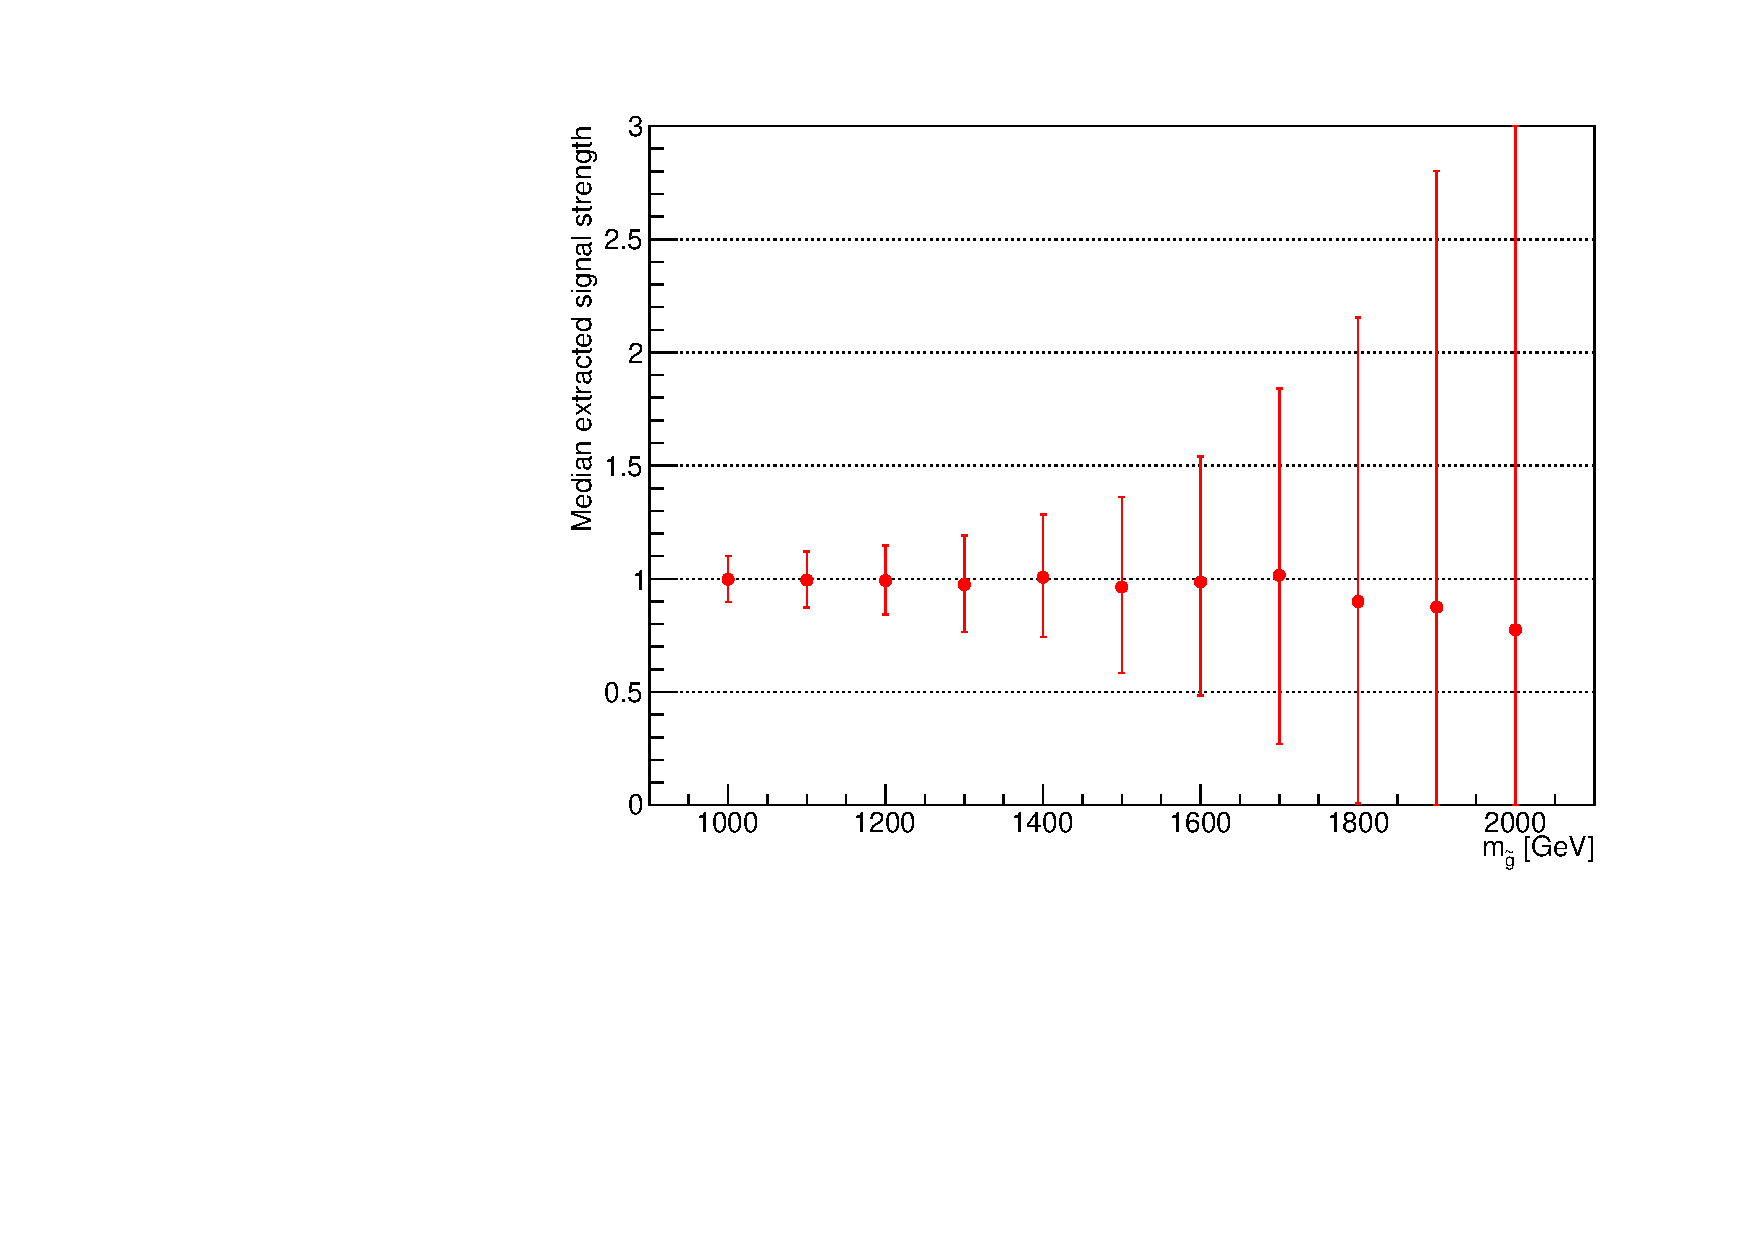
\includegraphics[angle=0,width=0.80\columnwidth]{fig/sig_injection.pdf}
\caption{Median extracted signal strength of 1,000 psuedodata experiments as a function of gluino mass.
The uncertainties drawn are the median upper and lower errors of the fitted signal strengths per mass point.}
\label{fig:sig_injection}
\end{figure}

\begin{figure}[tbp!]
\centering
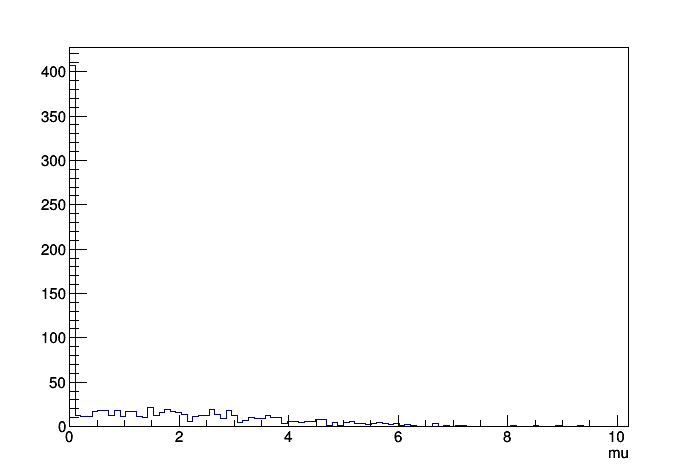
\includegraphics[angle=0,width=0.45\columnwidth]{fig/siginj_bias_1x.png}
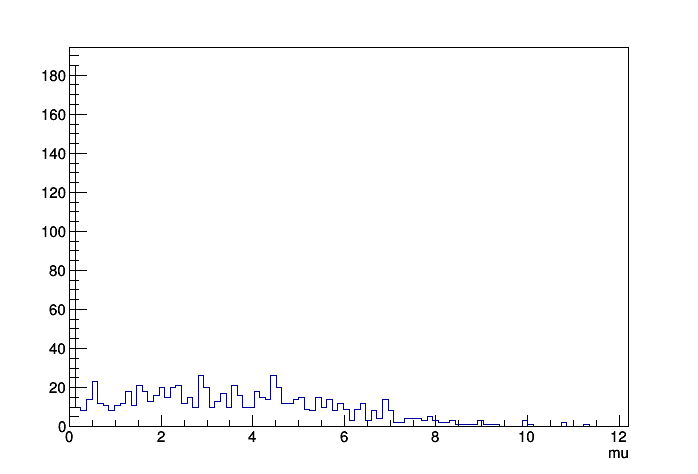
\includegraphics[angle=0,width=0.45\columnwidth]{fig/siginj_bias_3x.png}
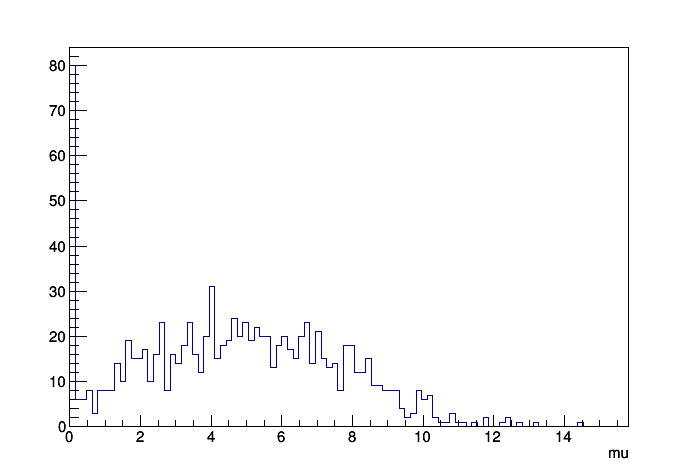
\includegraphics[angle=0,width=0.45\columnwidth]{fig/siginj_bias_5x.png}
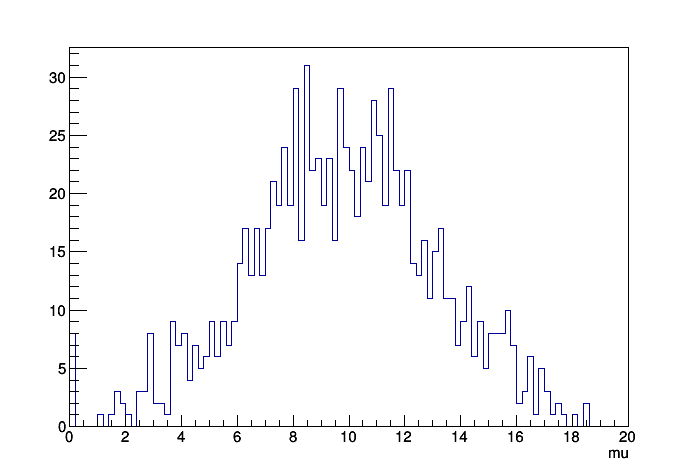
\includegraphics[angle=0,width=0.45\columnwidth]{fig/siginj_bias_10x.png}
\caption{Distribution of fitted signal strengths of 1000 psuedodata experiments for a 2000~\GeV gluino at 1x (top-left), 3x (top-right), 5x (bottom-left), and 10x (bottom-right) the nominal cross-section.
The amount of signal extracted is 78\%, 92\%, 95\%, and 98\% the injected signal, respectively.}
\label{fig:sig_injection}
\end{figure}

No modifications to the fit model are made to correct for this issue.
This is because the fit bias only affects mass points that are far above the highest mass (1650~\GeV) expected to be excluded by this analysis, and Figure~\ref{fig:sig_injection} shows that the fit bias is much smaller than the precision of the fit for those mass points.
Additionally, the coverage of the 95\% confidence intervals of the fit is tested using the signal injection experiments and found to be be either correct or slightly conservative, as shown in Table~\ref{tab:siginj_coverage}.

\begin{table}[tbp!]
\centering
\begin{tabular}{ |c|c|c| }
\hline
$\mglu = 1800~\GeV$ & $\mglu = 1900~\GeV$ & $\mglu = 2000~\GeV$ \\ \hline
$96\%$              & $95\%$              & $96\%$              \\ \hline
\end{tabular}
\caption{Actual coverage probability of the 95\% confidence interval of the fit for the mass points with a biased signal extraction.}
\label{tab:siginj_coverage}
\end{table}

\end{section}

\begin{section}{Control Region Fit}

While the signal injection studies are a useful validation of the fit model, it is important to validate the model using data in order to test for unmodelled effects.
To do this, the maximum-likelihood fit is performed with only the low-\Njets, low-\MJ control regions, as defined in Table~\ref{fig:analysis_regions}.
These bins are chosen due to their low-expected signal yields, which avoids signal contamination effects and unblinding the high-expected signal regions in the case further modification of the fit are needed.

The fit, under the background-only hypothesis, is able to model the observed data well, as seen in the post-fit \Nb distributions shown in Figure~\ref{fig:crfit}, without needing large adjustments to the nuisance parameters.
The change between the pre- and post-fit normalizations of the background processes is shown in Table~\ref{tab:crfit_norms}, while the pulls of the nuisance parameters corresponding to systematic uncertainties (largely controlling the shape of the \Nb distribution) are shown in Figure~\ref{fig:crfit_pulls}.
Both sets of values appear well-behaved, as the largest change in normalization is less than 50\%, with typical values around 10-15\%, while the nuisance parameters are all consistent with their pre-fit uncertainties, with most shifted less than 0.05~s.d.
The largest pulls correspond to nuisance parameters controlling the gluon splitting rate (gs, +0.42~s.d.), the light-flavor b-tag SFs (btag\_udsg, +0.37~s.d.), and the heavy-flavor b-tag SFs (btag\_bc, +0.13~s.d.).
These nuisances are expected to be shifted up as the observed data is higher than simulation in the tail of the pre-fit \Nb distributions, as seen in Figure~\ref{prefit_nb}.

\begin{figure}[tbp!]
\begin{center}
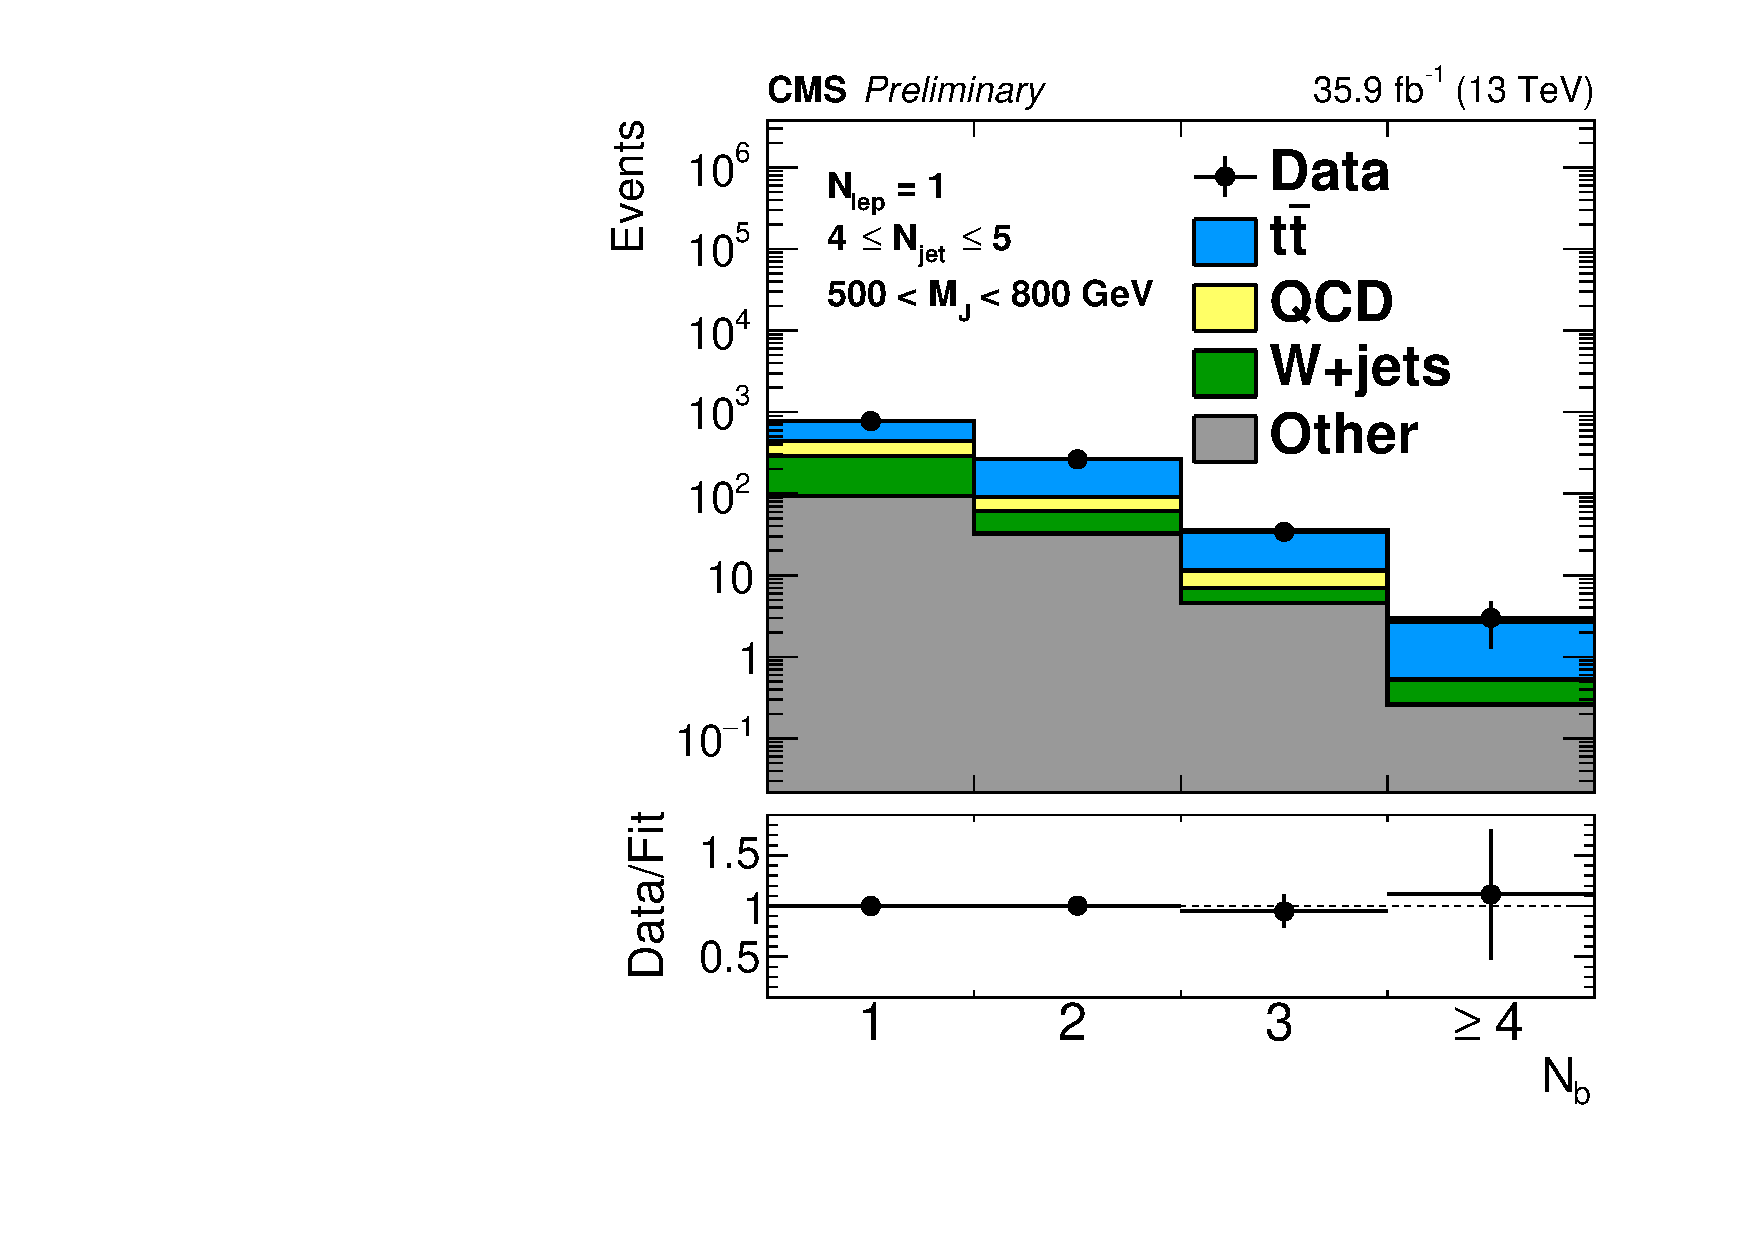
\includegraphics[angle=0,width=0.45\columnwidth]{fig/crfit_nlep1_nj45_lowmj.pdf}
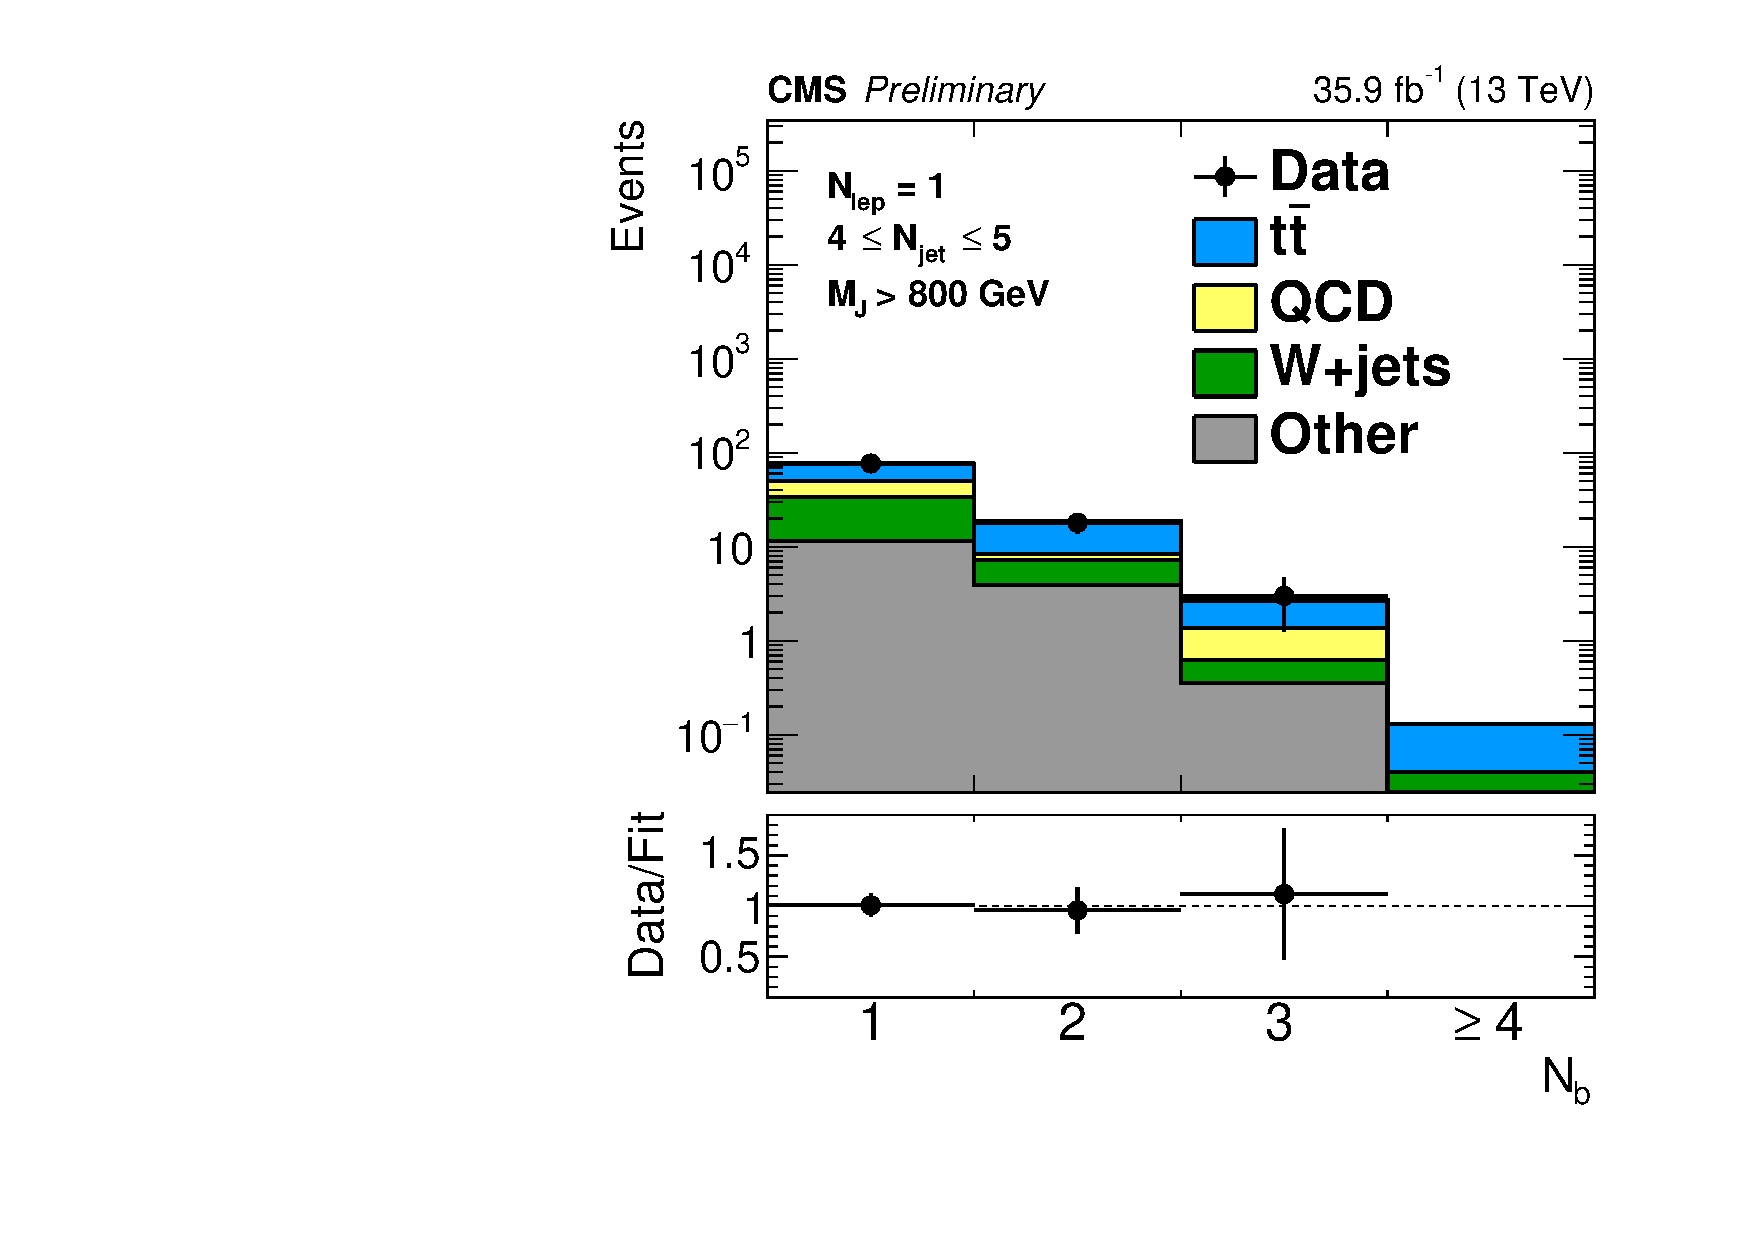
\includegraphics[angle=0,width=0.45\columnwidth]{fig/crfit_nlep1_nj45_highmj.pdf}
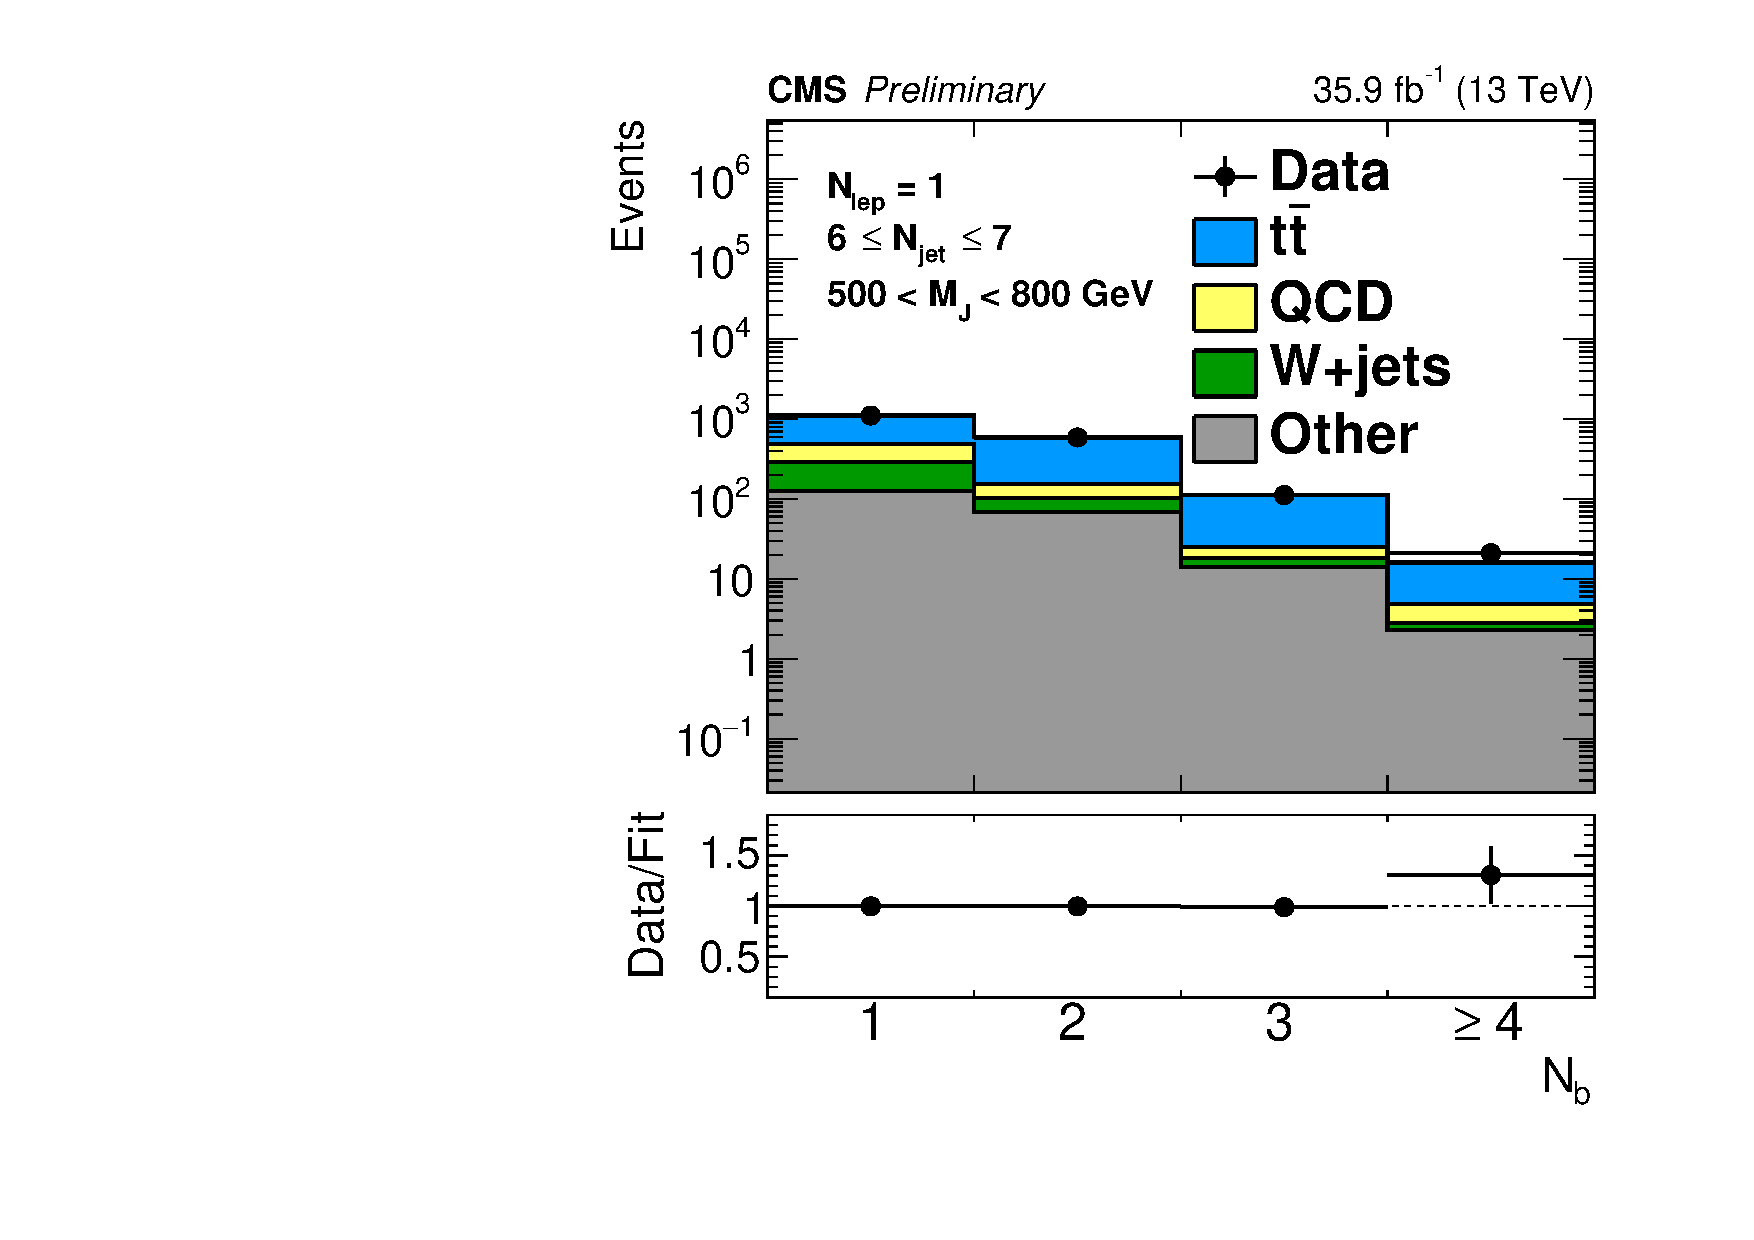
\includegraphics[angle=0,width=0.45\columnwidth]{fig/crfit_nlep1_nj67_lowmj.pdf}
\end{center}
\caption{Post-fit \Nb distributions of the control region fit.}
\label{fig:crfit}
\end{figure}

\begin{table}[tbp!]
\begin{center}
\begin{tabular}{|l|r|r|r|} \hline
Process   &   Pre-fit Yield   &  Post-fit Yield (b-only fit)   &   \% change \\
\hline
\hline
\multicolumn{4}{|c|}{$4 \leq \Njets \leq 5$, $500 \leq \MJ \leq 800$}         \\
\hline

\ttbar    &   501.4           &   $533.3  \pm  80.7$           &   +6.3      \\
QCD       &   218.8           &   $186.7  \pm  36.8$           &   -14.7     \\
\Wjets    &   400.4           &   $225.5  \pm  100.0$          &   -43.7     \\
Other     &   141.4           &   $131.8  \pm  34.5$           &   -6.8      \\

\hline
\multicolumn{4}{|c|}{$4 \leq \Njets \leq 5$, $\MJ \geq 800$}                 \\
\hline

\ttbar    &   36.9            &   $37.5   \pm  13.3$           &   +1.6      \\
QCD       &   23.1            &   $18.9   \pm  4.5$            &   -18.2     \\
\Wjets    &   45.7            &   $25.7   \pm  11.4$           &   -43.8     \\
Other     &   16.8            &   $15.7   \pm  3.8$            &   -6.5      \\

\hline
\multicolumn{4}{|c|}{$6 \leq \Njets \leq 7$, $500 \leq \MJ \leq 800$}        \\
\hline

\ttbar    &   1370.4          &   $1148.3 \pm  78.0$           &   -16.2     \\
QCD       &   293.9           &   $262.6  \pm  52.1$           &   -10.6     \\
\Wjets    &   367.7           &   $205.6  \pm  92.2$           &   -44.1     \\
Other     &   225.2           &   $209.7  \pm  58.5$           &   -6.9      \\
\hline
\end{tabular}
\caption{Table comparing the post-fit normalizations of the control region fit to the pre-fit yields for the various background processes.}
\label{tab:crfit_norms}
\end{center}
\end{table}


\begin{figure}[tbp!]
\begin{center}
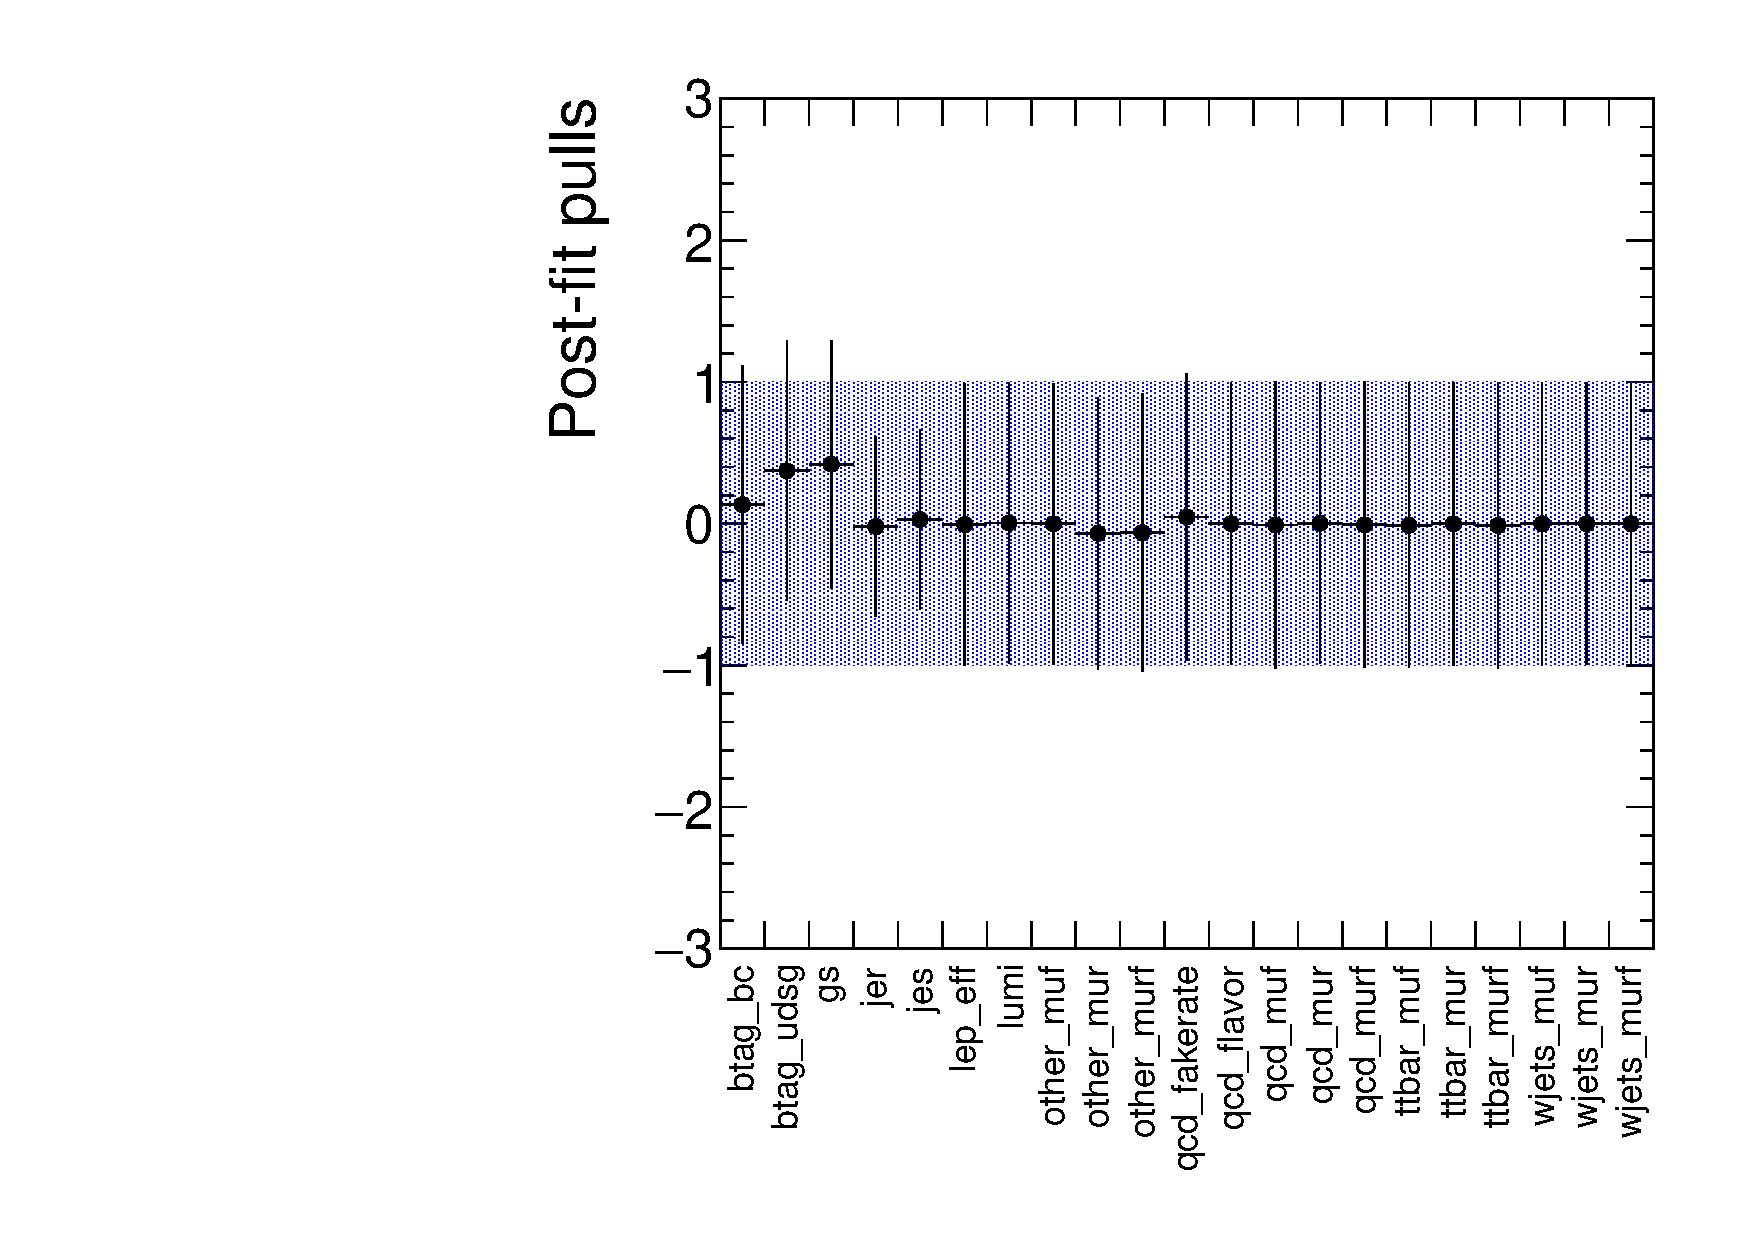
\includegraphics[angle=0,width=0.80\columnwidth]{fig/crfit_pulls.pdf}
\end{center}
\caption{Post-fit pulls of the background-only control region fit. 
The post-fit value of the nuisance parameter is indicated by the data point, while the post-fit uncertainty is shown as a black line and is normalized by the pre-fit uncertainty depicted as the blue band.}
\label{fig:crfit_pulls}
\end{figure}

Lastly, Table~\ref{tab:crfit_pulls} compares the post-fit pulls of the background-only and signal-plus-background control region fit.
The post-fit pulls between the two fits are fully consistent with each other, as is expected for these signal-poor regions.

\begin{table}[tbp!]
\begin{center}
\begin{tabular}{|l|r|r|r|} \hline
                                                  &  Post-fit pull     &  Post-fit pull     &                           \\
Nuisance parameter                                &  ($b$-only fit)    &  ($s+b$ fit)       &  $\rho(\theta_{i}, \mu)$  \\  \hline
b,c jet b-tag SF (btag\_bc)                       &  $+0.13 \pm 0.98$  &  $+0.07 \pm 1.05$  &  -0.18                    \\
u,d,s,g jet b-tag SF (btag\_udsg)                 &  $+0.37 \pm 0.92$  &  $+0.28 \pm 0.95$  &  -0.26                    \\
Gluon splitting (gs)                              &  $+0.42 \pm 0.87$  &  $+0.22 \pm 1.12$  &  -0.43                    \\
Jet energy resolution (jer)                       &  $-0.02 \pm 0.63$  &  $-0.02 \pm 0.60$  &  -0.01                    \\
Jet energy scale (jes)                            &  $+0.03 \pm 0.63$  &  $+0.03 \pm 0.61$  &  -0.03                    \\
Lepton efficiency (lep\_eff)                      &  $-0.01 \pm 0.99$  &  $-0.01 \pm 0.99$  &  +0.01                    \\   
Luminosity (lumi)                                 &  $+0.00 \pm 0.99$  &  $+0.00 \pm 0.99$  &  -0.01                    \\   
Fact. scale for other (other\_muf)                &  $-0.00 \pm 0.99$  &  $-0.00 \pm 0.99$  &  +0.00                    \\   
Renorm. scale for other (other\_mur)              &  $-0.07 \pm 0.96$  &  $-0.06 \pm 1.02$  &  +0.02                    \\   
Renorm. and Fact. scale for other (other\_murf)   &  $-0.06 \pm 0.98$  &  $-0.08 \pm 0.96$  &  +0.01                    \\   
QCD fake rate (qcd\_fakerate)                     &  $+0.05 \pm 1.01$  &  $+0.09 \pm 1.14$  &  +0.09                    \\   
Fact. scale for QCD (qcd\_muf)                    &  $-0.01 \pm 1.01$  &  $-0.01 \pm 1.01$  &  -0.00                    \\   
Renorm. scale for QCD (qcd\_mur)                  &  $+0.00 \pm 0.99$  &  $+0.00 \pm 0.99$  &  -0.00                    \\   
Renorm. and Fact. scale for QCD (qcd\_murf)       &  $-0.01 \pm 1.01$  &  $-0.01 \pm 1.01$  &  -0.00                    \\   
Fact. scale for \ttbar (ttbar\_muf)               &  $-0.01 \pm 1.01$  &  $-0.01 \pm 1.00$  &  +0.00                    \\   
Renorm. scale for \ttbar (ttbar\_mur)             &  $-0.00 \pm 1.00$  &  $+0.00 \pm 0.99$  &  +0.01                    \\   
Renorm. and Fact. scale for \ttbar (ttbar\_murf)  &  $-0.01 \pm 1.01$  &  $-0.01 \pm 1.00$  &  +0.01                    \\   
Fact. scale for \Wjets (wjets\_muf)               &  $-0.00 \pm 0.99$  &  $+0.00 \pm 0.99$  &  +0.00                    \\   
Renorm. scale for \Wjets (wjets\_mur)             &  $-0.00 \pm 0.99$  &  $-0.00 \pm 0.99$  &  -0.00                    \\   
Renorm. and Fact. scale for \Wjets (wjets\_murf)  &  $-0.00 \pm 1.00$  &  $-0.00 \pm 1.00$  &  +0.00                    \\   
\hline
\end{tabular}
\caption{Table of post-fit pulls of the background-only and signal-plus-background control region fit.
The last column, $\rho(\theta_{i}, \mu)$, lists the correlation between the corresponding nuisance parameter, $\theta_{i}$, and the nuisance parameter controlling the signal strength, $\mu$.}
\label{tab:crfit_pulls}
\end{center}
\end{table}

\end{section}
